% !TeX spellcheck = en_US
\todo{what's done from the concept}
\todo{still high-level}
\todo{what problem is solved?}

\begin{itemize}
	\item implemented db concept
		\subitem picture from simple-sbml-demo
		\subitem rest of pictures in appendix
	\item Ontology import
		\subitem changes to \masymos core
		\subitem using existing import mechanics, but dynamic
	\item http server storage concept?
\end{itemize}

solved:
"A model VCS should be tailored to existing model representation formats, which are typically XML and RDF based. It should furthermore reflect the temporal evolution of a model and present model changes to the users." \citep{Waltemath2013}

The objective of this thesis is therefore to investigate into a concept to store systems biology models in a way, that multiple versions can be accessed, queried, and compared. Further, semantical annotations of changes between these versions shall be introduced. These additional relations are meant to improve the ability to query for a version of a model by specific criteria and consequently improving the user experience for biologists seeking to build onto existing models, as the evolution of them plays an important role for them \citep{Scharm2015}

\begin{figure}
	\centering
	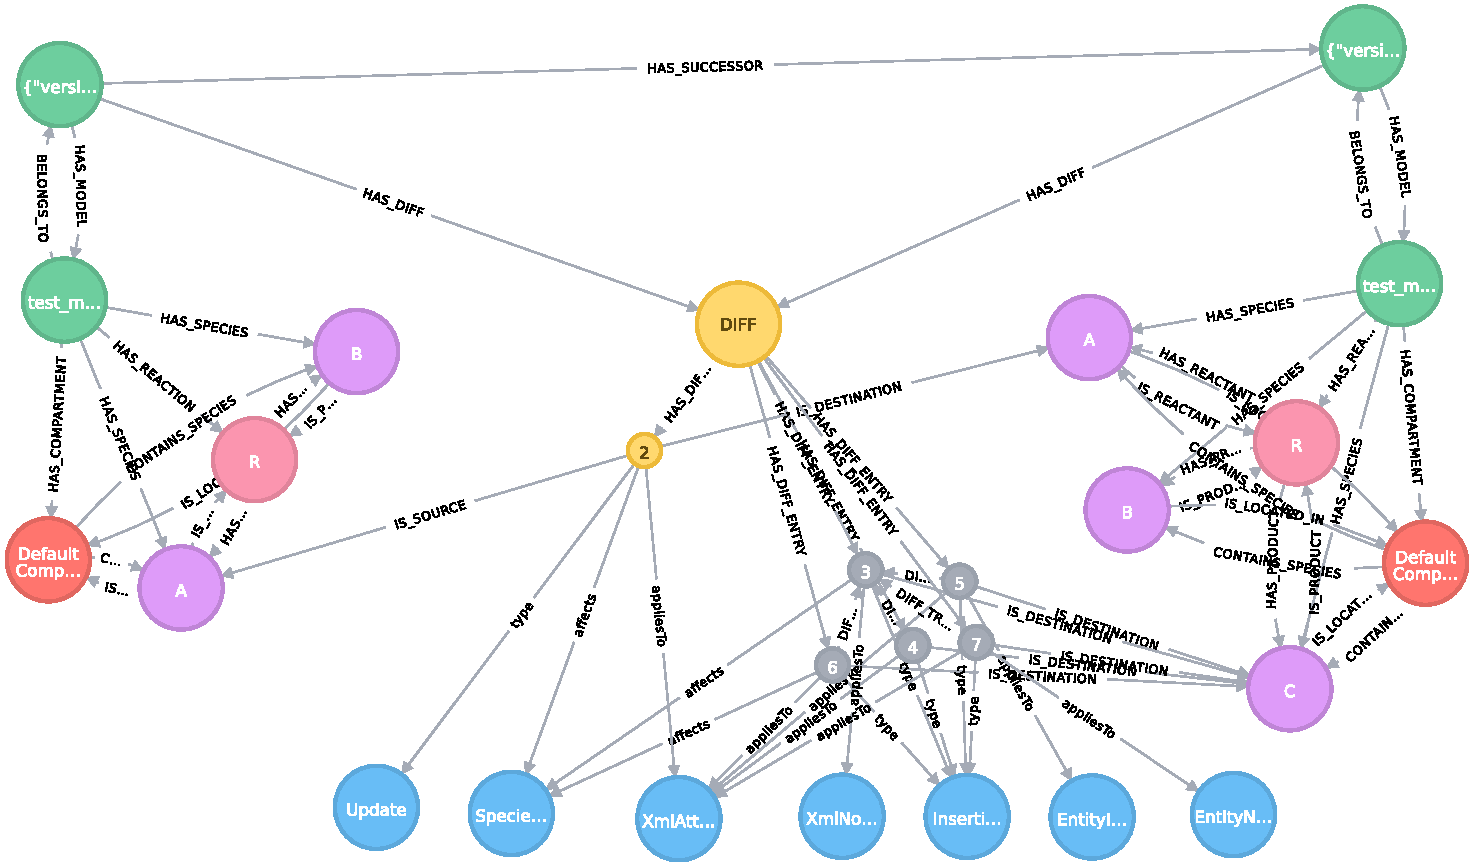
\includegraphics[width=\textwidth]{resources/neo4j-renders/demo-sbml-simple-diff.pdf}
	\caption{Reduced representation of a delta in \masymos, between two versions of a the simple \sbml demo model}
	\label{fig:results:simple-diff}
\end{figure}